	\documentclass[10pt,oneside]{CBFT_book}
	
	% Algunos paquetes
	\usepackage{amsmath}
	\usepackage{amssymb}
	\usepackage{graphicx}
	\usepackage{libertine}
%   	\usepackage[bold-style=TeX]{unicode-math}
  	\usepackage[ math-style=TeX, bold-style=ISO ]{unicode-math}
% 	Este package es el que configura cómo salen las cosas en negrita, y en general
% 	en math mode.
  	
	\usepackage{lipsum}

	\usepackage[numbers]{natbib}
	\setcitestyle{square}


	\usepackage{polyglossia}
	\setdefaultlanguage{spanish}

	\usepackage{CBFT.estilo} % Cargo la hoja de estilo
	

	% Tipografías
	% \setromanfont[Mapping=tex-text]{Linux Libertine O}
	% \setsansfont[Mapping=tex-text]{DejaVu Sans}
	% \setmonofont[Mapping=tex-text]{DejaVu Sans Mono}

	%===================================================================
	%	DOCUMENTO PROPIAMENTE DICHO
	%===================================================================

% \title{CBFT Mecánica clásica}
% \author{Mecánica lagrangiana}
% \date{\today}

\begin{document}
% \maketitle
% \tableofcontents
\chapter{Mecánica newtoniana}

Tal vez sea una simplificación, pero no una muy terrible, decir que el curso de mecánica clásica
busca reemplazar la mecánica basada en las ecuaciones de Newton,
\[
	\vb{F} = m \vb{a} 
\]
por un \emph{formalismo} más poderoso y que se podrá aplicar luego a otros campos.
Este formalismo es el corazón de la mecánica clásica.

\begin{figure}[hbt]
	\begin{center}
	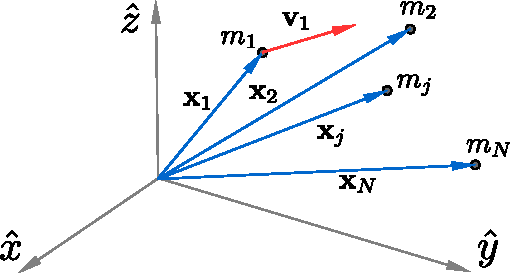
\includegraphics[width=0.6\textwidth]{images/fig_mc_leyes_cons.pdf}
	\end{center}
	\caption{Sistema de partículas de masas $m_i$ con sus correspondientes vectores de
	posición $\vb{x}_i$. La partícula $m_1$ tiene además indicado su vector velocidad $\vb{v}_1$.}
	\label{fig_mc_leyes_cons}
\end{figure} 


% =================================================================================================
\section{Momento angular}
% =================================================================================================



\[
	\vb{L} = \vb{r} \times \vb{p}
\]
\begin{figure}[hbt]
	\begin{center}
	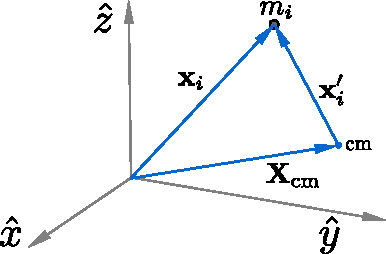
\includegraphics[width=0.6\textwidth]{images/fig_mc_angularmom.pdf}	
	\end{center}
	\caption{}
\end{figure} 
\[
	\vb{r}_i = \vb{R} + \vb{r}_i' \qquad \vb{v}_i = \vb{V} + \vb{v}_i'
\]
\[
	\vb{L}^T_O = \sum_i \vb{r}_i \times \vb{p}_i = \sum_i (\vb{R} + \vb{r}_i') \times m_i (\vb{V} + \vb{v}_i')
\]
\[
	\vb{L}^T_O = \sum_i ( \vb{R} \times m_i \vb{V}  + \vb{R} \times m_i \vb{v}_i'
	+ \vb{r}_i' \times m_i \vb{V} 	+ \vb{r}_i' \times m_i \vb{v}_i' )
\]
pero si recordamos que se cumplen 
\[
	\vb{R} = \sum_i \frac{m_i \vb{r}_i}{M}
\]
\[
	M\vb{R} = \sum_i m_i (\vb{R} + \vb{r}_i') = \sum_i m_i \vb{R} + \sum_i m_i \vb{r}_i'
\]
\[
	M\vb{R} = M \vb{R} + \sum_i m_i \vb{r}_i' \quad \Longrightarrow 0 = \sum_i m_i \vb{r}_i'
\]
podemos volver a las ecuaciones anteriores para poner
\[
	\vb{L}^T_O = \vb{R} \times M \vb{V}  + \vb{R} \times \frac{d}{dt}\left( m_i \vb{r}_i' \right)
	+ \left( \sum_i m_i \vb{r}_i' \right) \times \vb{V} + \sum_i \vb{r}_i' \times m_i \vb{v}_i'
\]
\[
	\vb{L}^T_O = \vb{R} \times M \vb{V}  + \sum_i \vb{r}_i' \times m_i \vb{v}_i'
\]
\[
	\vb{L}^T_O = \vb{L}^{cm} + \vb{L}^{sist}_{cm}
\]
siendo el primer término del lado derecho el momento angular orbital y el segundo el momento angular
de spin.

Con respecto a la conservacion del momento angular, se tendrá
\[
	\dtot{\vb{L}_O}{t} = \sum \vb{\tau}_O
\]
que se puede ver como suma del torque de fuerzas externas y de fuerzas internas. En el primer caso,
los torques externos sumarán cero si las fuerzas externas son nulas o centrales.
En el segundo caso los torques internos son nulos si vale el principio de acción y reacción fuerte;
es decir si
\[
	\vb{r}_i - \vb{r}_j \parallel F_{ij}.
\]

% =================================================================================================
\section{Trabajo y energía}
% =================================================================================================


Sólo las componentes tangenciales de la fuerza producen trabajo.

Consideremos una partícula de masa $ m $ que se mueve sobre una cierta trayectoria suave, ver {Figura} 
\ref{fig_mc_workenergy}, debido a la acción de una fuerza \vb{F}.
Su velocidad \vB{v} es en todo momento tangente a la trayectoria y define de esta forma un versor $ \hat{t} $
colineal con la misma. Asimismo podemos definir un versor $ \hat{n} $ normal a la trayectoria.
Descomponiendo la fuerza y la velocidad en estas dos direcciones, se tiene 
\[
	\vb{F} = F_{\hat{t}} \hat{t}  + F_{\hat{n}} \hat{n} \qquad \qquad \vB{v} = v_{\hat{t}} \: \hat{t}
\]
de manera que la segunda ley de Newton 
\[
	m \dtot{\vB{v}}{t} = \vb{F}
\]
en la componente $\hat{t}$ es
\[
	m \dtot{v}{t} = F_{\hat{t}}
\]
donde hemos despojado del subíndice a $v$. Involucrando al diferencial de arco $ ds = | d\vb{x} | $ a lo largo de la 
trayectoria es
\[
	m \: dv \:\dtot{s}{t} = m \: v \: dv = F_{\hat{t}} \: ds = \vb{F} \cdot d\vb{x},
\]
donde la última igualdad se ha escrito en virtud de que $ F_{\hat{n}} \perp d\vb{x} $ siempre.

\begin{figure}[hbt]
	\begin{center}
	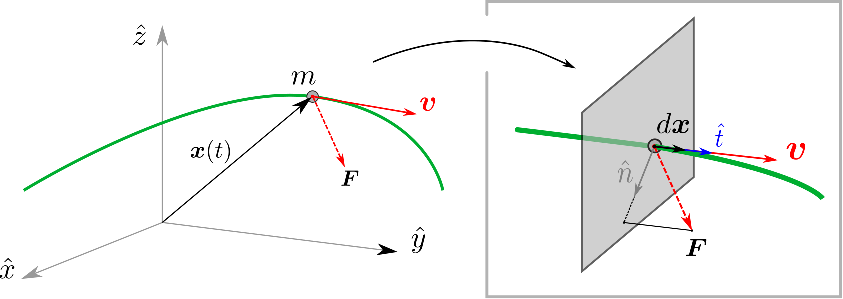
\includegraphics[width=0.9\textwidth]{images/fig_mc_workandenergy.pdf}	
	\end{center}
	\caption{}
	\label{fig_mc_workenergy}
\end{figure} 

Podemos integrar ambos miembros de la anterior ecuación entre $\vB{x}(t_0) \equiv \vB{x}_0$ y su 
correspondiente velocidad $v(t_0) \equiv v_0$ hasta $\vB{x}, \vB{v}$, 
\[
	m \int_{v_0}^v \: v \: dv = \int_{\vB{x}_0}^{\vB{x}}  \vb{F} \cdot d\vb{x}
\]
obteniendo
\[
	\left. \frac{1}{2} m v^2 \right|_{v_0}^v = W_{\vB{x}_0 \to \vB{x}} 
\]
que es el llamado \emph{teorema de las fuerzas vivas} para una partícula de masa $m$ y nos dice que la
variación de energía cinética en la trayectoria es igual al trabajo de todas las fuerzas que actúan
sobre la misma,
\[
	\Delta T = W.
\]

En el caso particular en que la fuerza sea normal en toda la trayectoria integrada se tendrá $\Delta T = 0 $,
es decir se conserva la energía cinética a lo largo de toda la trayectoria. El trabajo de una fuerza
está asociado a las componentes tangenciales de la fuerza; las componentes normales no hacen trabajo.

\notamargen{ Falta meter lo de \[ 	 m \frac{v^2}{\rho} = F_n \] }

Si la fuerza proviene de un potencial\footnote{El menos delante del gradiente es una convención, como se verá a
continuación}, se tiene 
\be
	\vB{F} = - \nabla V
	\label{fuerza_prov_potencial}
\ee
y podemos expresar en coordenadas cartesianas esta equivalencia \eqref{fuerza_prov_potencial}
\[
	\vB{F} = -\left( \dpar{V}{x_1}, \dpar{V}{x_2}, \dpar{V}{x_3} \right)
\]
y evaluar la integral del trabajo para obtener
\[
	W = \int_{\vB{x}_0}^{\vB{x}_1}  \vb{F} \cdot d\vb{x} =
	\int_{t_0}^{t_1}  \vb{F}(\vB{x}[t]) \cdot \dotvB{ x } \: dt =
	- \int_{t_0}^{t_1}  \sum_{k=1}^3 \left[ \dpar{V}{x_k} \dtot{x_k}{t} \right] \: dt =
	\Phi_0 - \Phi_1
\]
lo cual significa que la integral es independiente de la trayectoria $\vB{x}_0 \to \vB{x}_1$.

Entonces, juntando
\[
% 	\underbrace{T_1 - T_0 = W_{0 \to 1}}_{\text{Vale siempre}} = \Phi_0 - \Phi_1 
	\rlap{ $\overbrace{\phantom{T_1 - T_0 = W_{0 \to 1}}}^{\text{Vale siempre}} $}  T_1 - T_0 =
	\underbrace{ W_{0 \to 1} = \Phi_0 - \Phi_1 }_{\text{Si $\vB{F}$ proviene de potencial} }
\]
y pasando de miembros
\[
	(T_1 + \Phi_1) = (T_0 + \Phi_0 ) 
\]
se tiene que la cantidad $ E = T + V $ (la energía mecánica) se conserva si la fuerza $\vB{F}$ proviene de un 
potencial $V$.

Notemos que el versor desplazamiento $d\vb{s}$ {\it camina} por la trayectoria.

\[
	W = W^{ext} + W^{int}
\]
y entonces como el trabajo externo viene de 
\[
	\sum_i^N \int \vb{F}^{ext}_i \cdot d\vb{s}_i
\]
necesito $\vb{F}_i = \vb{F}_i(\vb{r}_i)$ y $\nabla \times \vb{F}_i=0$.
Para el trabajo interno
\[
	W_i^{int} = \int \sum_j^N  \vb{F}_{ij} \cdot d\vb{s}_i
\]
\[
	W^{int} = \sum_i \int \sum_j  \vb{F}_{ij} \cdot d\vb{s}_i
\]
\[
	\frac{1}{2} \sum_i \sum_j \int \vb{F}_{ij} \cdot d\vb{s}_i + \vb{F}_{ji} \cdot d\vb{s}_j =
	\frac{1}{2} \sum_i \sum_j \int \vb{F}_{ij} \cdot \left( d\vb{s}_i - d\vb{s}_j \right)
\]

% =================================================================================================
\section{Definiciones}
% =================================================================================================

El número de grados de libertad es el número de coordenadas independientes para resolver el problema.
Las fuerzas de vínculo $F^v$ se {\it acomodan} en todo momento para satisfacer las ligaduras.
Entonces las $\vb{F}^v$ son perpendiculares a los desplazamientos compatibles con los vínculos de
manera que 
\[
	W_{F^v} = 0
\]
\begin{figure}[hbt]
	\begin{center}
	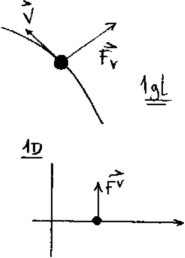
\includegraphics[width=0.3\textwidth]{images/fig_mc_vinculos1.pdf}	 
	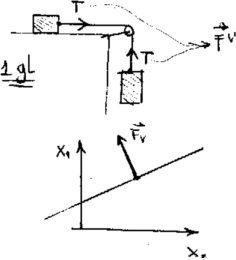
\includegraphics[width=0.3\textwidth]{images/fig_mc_vinculos2.pdf}
	\end{center}
	\caption{}
\end{figure} 

Los vínculos se clasifican en
\[
\textrm{holónomos} 
\begin{Bmatrix}
 f(r_i,t) = 0 \qquad \textrm{reónomos} \\
\; f(r_i) = 0 \qquad \textrm{esclerónomos} \;\\
\end{Bmatrix} 
\]
los cuales cumplen que  $W_{virtual}^{F^v}=0$, y
\[
\textrm{no holónomos} 
\begin{Bmatrix}
 f(r_i,t) \geq 0  \\
 f(r_i) \geq cte. \quad f(\dot{r}_i) = 0  \; \\
\end{Bmatrix}
\]
los cuales no cumplen, en general, que $\vb{F}^v$ perpendicular al desplazamiento posible.
\begin{figure}[hbt]
	\begin{center}
	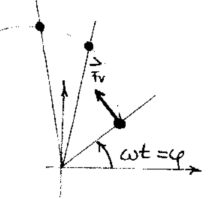
\includegraphics[width=0.3\textwidth]{images/fig_mc_vinculos3.pdf}	
	\end{center}
	\caption{}
\end{figure} 
donde un desplazamiento virtual es un desplazamiento a $t_0$ fijo compatible con los vínculos,
mientras que un desplazamiento real es un desplazamiento en $\delta t$ durante el cual varían
fuerzas y ligaduras.

A tiempo fijo el desplazamiento es en $\hat{r} \perp \vb{F}^v$.

\[
	f(x_i,t) = cte. \Longrightarrow \sum_i^N \dpar{f}{x_i} \delta x_i + \dpar{f}{t} \delta t = 0 
\]
o bien
\[
	\nabla f \cdot \vb{\delta r} = 0
\]
% Como ejemplo citamos \cite{einstein}.
% O bien \cite{example}.
% Tal vez \citep{Aspnes:1973}

% ============================================================================

% \bibliographystyle{CBFT-apa-good} % (uses file "apa-good.bst")
% \bibliography{CBFT.Referencias} % La base de datos bibliográfica


\end{document}
